\documentclass[12pt]{iopart}
\usepackage{graphicx}
\usepackage{hyperref}
\usepackage{cite}
\usepackage{booktabs}
\usepackage{qrcode}
\usepackage{amssymb}

\expandafter\let\csname equation*\endcsname\relax
\expandafter\let\csname endequation*\endcsname\relax
\usepackage{amsmath}

\providecommand{\mathbb}[1]{\mathbf{#1}}

\begin{document}
	
	\title{Resonance Field Theory: Axiomatics, Fundamental Formula, and
		Empirical Validation}
	
	\author{Dominic-Ren\'e Schu}
	\address{Independent Researcher, Germany\\
		\href{https://github.com/DominicReneSchu/RFT}%
		{https://github.com/DominicReneSchu/RFT}\\
		ORCID: 0009-0004-9769-9061\\
		Email: dominic.rene.schu@gmail.com}
	
	\begin{abstract}
		Resonance Field Theory (RFT) is presented as an axiomatic framework
		that describes oscillatory coupling as a universal organizing principle
		of physical and systemic phenomena. From seven axioms follows a
		parametric extension of the Planck relation by a phase-dependent
		coupling operator $\varepsilon(\Delta\varphi) \in [0,1]$:
		$E = \pi \cdot \varepsilon(\Delta\varphi) \cdot \hbar \cdot f$.
		The theory is empirically validated across four independent domains:
		(1)~$1{,}500{,}000$~Monte Carlo simulations on CMS Open Data
		dielectron events detect five known particle resonances
		($\phi$(1020), J/$\psi$, $\Upsilon$(1S), $\Upsilon$(2S), Z boson)
		with empirical p-value~$= 0$, stable across three KDE bandwidths and
		ten seeds;
		(2)~$1{,}530$~coupled FLRW simulations in which the coupling
		efficiency $\eta(\Delta\varphi) \approx \cos^2(\Delta\varphi/2)$
		follows as an emergent property, with scaling
		$\mathrm{d}d_\eta/\mathrm{d}H_0
		= (0.00113 \pm 0.00017)$~(km/s/Mpc)$^{-1}$
		and improvement $\Delta\chi^2 = +16$ compared to
		Planck-2018 CMB data;
		(3)~Resonance reactor simulation with $\kappa = 1$ (no free
		parameter) and fission break-even $Q \approx 1.0$;
		(4)~ResoTrade, axiomatically developed over 12~versions, achieves
		$+26.3\%$ vs.\ HODL over 24~months across 4~market regimes, with
		live validation since February 2026 ($+4.13\%$ in 5~days) and a
		falsification test over $200{,}000$~altcoin episodes. Each of the
		7~axioms is individually validated on the market.
		Two falsifiable experimental proposals are presented:
		(I)~phase-dependent photo-excitation of Am-241 at ELI-NP
		(nuclear physics, 0~free parameters, $>50{,}000\,\sigma$) and
		(II)~center-of-mass shift of a ${}^{87}$Rb BEC in a harmonic trap
		(quantum mechanics, 1~free parameter~$\lambda$). Both experiments
		test the coupling function $\cos^2(\Delta\varphi/2)$ over
		19~orders of magnitude in energy and are independently falsifiable.
		All derivations, source codes, and data are openly available at
		\url{https://github.com/DominicReneSchu/RFT}.
	\end{abstract}
	
	\noindent\textbf{Keywords:} resonance, field theory,
	coupling operator, axiomatics, Monte Carlo simulation,
	FLRW cosmology, Giant Dipole Resonance, transmutation,
	algorithmic trading, empirical validation, open science
	
	\medskip
	
	\noindent\textbf{Data and Code Availability:}
	\url{https://github.com/DominicReneSchu/RFT}
	
	
	%% ============================================================
	\section{Introduction}
	%% ============================================================
	
	Modern physics possesses formalisms of enormous predictive
	power, yet its conceptual foundations remain fragmented.
	Quantum mechanics, relativity theory, and thermodynamics
	operate in separate theoretical spaces. Programs of quantum
	gravity increase mathematical complexity without creating
	empirical testability.
	
	This manuscript introduces \textit{Resonance Field Theory}
	(RFT) -- an axiomatic framework that postulates oscillatory
	coupling as the primary organizing principle of physical
	systems. RFT formulates seven axioms from which follow a
	parametric extension of quantum mechanics, a unified
	differential equation structure, and testable predictions.
	
	Unlike existing approaches, RFT does not aim at a
	unification of the fundamental forces, but rather at a
	conceptual framework that describes resonance phenomena
	uniformly across scales and domains -- from particle physics
	through cosmology and nuclear technology to financial markets.
	
	The manuscript is structured as follows: Section~2
	formulates the seven axioms. Section~3 develops the
	mathematical structure. Section~4 presents the empirical
	validation across four domains: particle physics (Monte
	Carlo on CMS data), cosmology (coupled FLRW simulations
	with Planck-2018 comparison), nuclear technology (resonance
	reactor), and financial markets (ResoTrade). Section~5
	discusses the comparison with established theories.
	Section~6 presents two falsifiable experimental proposals.
	Section~7 identifies open questions. Section~8 summarizes.
	
	
	%% ============================================================
	\section{Axiomatic Foundations}
	%% ============================================================
	
	RFT is based on seven hierarchically structured axioms.
	The axioms are not independent but constitutively
	intertwined: A1--A3 define the oscillatory structure,
	A4 the energetics, A5--A6 the dynamics, A7 the stability.
	
	\subsection{Axiom 1: Universal Oscillation}
	
	Every physical entity is describable by an oscillation
	function:
	\begin{equation}
		\psi(x, t) = A \cos(kx - \omega t + \phi)
		\label{eq:oscillation}
	\end{equation}
	
	\textit{Example:} Quantized electron orbitals, pendulum with
	natural frequency, circadian rhythms, market cycles,
	Giant Dipole Resonance in atomic nuclei.
	In ResoTrade: AC/DC decomposition of the BTC price field
	($\psi_{\mathrm{price}} = \mathrm{DC}_{168h}
	+ \mathrm{AC}$).
	
	\subsection{Axiom 2: Superposition and Interference}
	
	Oscillations superpose linearly:
	\begin{equation}
		\Psi(x, t) = \sum_i \psi_i(x, t)
		\label{eq:superposition}
	\end{equation}
	
	\textit{Example:} Double-slit interference,
	beating phenomena, AC/DC decomposition of price fields,
	GDR double-peak structure in deformed nuclei.
	In ResoTrade: Three superposed modes
	($e_{\mathrm{short}}$, $e_{\mathrm{long}}$,
	experience memory) systematically generate more
	information than any single mode.
	
	\subsection{Axiom 3: Resonance Condition}
	
	Coupling between two systems occurs when their
	frequencies stand in rational ratio:
	\begin{equation}
		\frac{f_1}{f_2} = \frac{n}{m}, \quad
		n, m \in \mathbb{Z}^+
		\label{eq:resonance_condition}
	\end{equation}
	
	\textit{Example:} Molecular orbital resonance,
	Tacoma Narrows bridge. Negative test: altcoins without
	natural frequency produce no resonance
	($200{,}000$~episodes, draw rate $98.4\%$).
	In the resonance reactor: excitation frequency equals
	the GDR frequency of the nucleus.
	In ResoTrade: $\mathrm{MA}_{\mathrm{SHORT}}$ (24h)
	and $\mathrm{MA}_{\mathrm{LONG}}$ (168h) stand in
	ratio $1{:}7$.
	
	\subsection{Axiom 4: Coupling Energy}
	
	The energy transferred by resonance is:
	\begin{equation}
		E = \pi \cdot \varepsilon(\Delta\varphi) \cdot \hbar \cdot f
		\label{eq:grundformel}
	\end{equation}
	with the phase-dependent coupling operator
	$\varepsilon(\Delta\varphi) \in [0,1]$, where
	$\Delta\varphi$ denotes the phase difference between
	coupled systems.
	
	\textbf{Dimensional analysis:}
	$[\,] \cdot [\,] \cdot [\mathrm{J{\cdot}s}] \cdot
	[\mathrm{s}^{-1}] = [\mathrm{J}]$ $\checkmark$
	
	\textbf{Planck special case:}
	For $\varepsilon = 1/(2\pi)$ it follows that
	$E = \frac{1}{2}\hbar f$, consistent with the
	ground-state energy of the harmonic oscillator.
	
	\textbf{Limiting values:}
	\begin{itemize}
		\item $\varepsilon = 0$: no coupling
		(destructive interference)
		\item $\varepsilon = 1$: maximum coupling
		(complete phase coherence)
	\end{itemize}
	
	\textit{In ResoTrade:} Downtrend pause gate --
	when the DC component falls sharply,
	$\varepsilon \to 0$. The system pauses and achieves
	exactly $+44.9\%$ vs.\ HODL in this phase.
	
	\subsection{Axiom 5: Energy Direction}
	
	Energy is a vectorial quantity with magnitude and
	direction in the resonance field:
	\begin{equation}
		\vec{E}_{\mathrm{dir}} =
		E_{\mathrm{short}} - E_{\mathrm{long}}
		\label{eq:energy_direction}
	\end{equation}
	
	The energy direction vector determines the dynamics of
	energy flow. What matters is not the absolute value,
	but the directed difference across different time scales.
	
	\textit{In ResoTrade:}
	\texttt{energy\_dir = e\_short - e\_long} determines
	the trading direction. All scalar indicators
	(RSI, Momentum, MA-crossover) have
	correlation~$< 0.05$ with future price movements.
	The energy direction vector, by contrast,
	systematically identifies the direction of capital flow.
	
	\subsection{Axiom 6: Information Flow through
		Resonance Coupling}
	
	Information propagates exclusively along coherent
	resonance paths. Information transfer requires
	phase and frequency synchronization.
	\begin{equation}
		\mathrm{Information\;flow} \iff
		\mathrm{Phase\textrm{-}\;and\;frequency\;synchronization}
		\label{eq:information}
	\end{equation}
	
	\textit{In ResoTrade:} Resonance gate -- trades only
	with phase coherence between action and energy direction.
	Approximately 40\% of all policy proposals are blocked
	as anti-resonant. In live operation:
	97\% of all cycles are recognized as non-resonant (HOLD).
	
	\subsection{Axiom 7: Invariance}
	
	Resonance structures are preserved under variation of
	the observer perspective and system parameters:
	\begin{equation}
		\forall\; T : \mathcal{R} \to \mathcal{R}', \quad
		\mathrm{Structure}(\mathcal{R})
		= \mathrm{Structure}(\mathcal{R}')
		\label{eq:invariance}
	\end{equation}
	
	\textit{Example:} Monte Carlo results stable over
	$50{,}000$ runs. ResoTrade positive in
	4/4~market regimes with identical parameters.
	
	
	%% ============================================================
	\section{Mathematical Formulation}
	%% ============================================================
	
	\subsection{Fundamental Formula and Coupling Operator}
	
	The central equation~(\ref{eq:grundformel}) extends the
	Planck relation $E = \hbar\omega$ by a coupling term.
	The factor $\pi$ reflects the cyclic geometry of
	resonance coupling. The operator
	$\varepsilon(\Delta\varphi)$ is determined from the phase
	relationship of the concrete system.
	
	For a system with phase difference $\Delta\varphi$
	between excitation and response, the simplest model is:
	\begin{equation}
		\varepsilon(\Delta\varphi) =
		\frac{1}{2}(1 + \cos\Delta\varphi)
		= \cos^2(\Delta\varphi/2)
		\label{eq:epsilon_cos}
	\end{equation}
	This gives $\varepsilon = 1$ at $\Delta\varphi = 0$
	(resonance) and $\varepsilon = 0$ at
	$\Delta\varphi = \pi$ (anti-resonance).
	
	\subsection{Identity between Operator and Observable}
	\label{sec:eps_eta}
	
	In the FLRW simulation the coupling efficiency
	$\eta(\Delta\varphi)$ emerges as a measurable cross term.
	The analytical expectation is
	$\eta_{\mathrm{theo}} = \cos^2(\Delta\varphi/2)$.
	Since simultaneously the theoretical coupling operator
	$\varepsilon(\Delta\varphi) = \cos^2(\Delta\varphi/2)$
	holds, the exact identity follows:
	\begin{equation}
		\varepsilon(\Delta\varphi)
		= \eta(\Delta\varphi)
		= \cos^2(\Delta\varphi/2)
		\label{eq:eps_eta_identity}
	\end{equation}
	This identity has an immediate consequence for the
	resonance reactor: the coupling strength parameter
	in the effective decay rate
	$\lambda_{\mathrm{eff}} = \lambda_0 + \eta \cdot \kappa
	\cdot \Phi_\gamma \cdot \sigma$ is not a free parameter,
	but exactly $\kappa = 1$.
	
	\subsection{Resonance Differential Equation (rDE)}
	
	RFT unifies classical differential equations as
	special cases of a general resonance coupling relation:
	\begin{equation}
		\mathcal{R}(x, \dot{x}, \ddot{x}, t, \Phi) = 0
		\label{eq:rdgl}
	\end{equation}
	where $\Phi$ describes the coupling term. Special cases:
	
	\medskip
	\begin{center}
		\begin{tabular}{lll}
			\hline
			\textbf{System} & \textbf{Coupling $\Phi$}
			& \textbf{Equation} \\
			\hline
			Harm.\ Oscillator & $-\omega_0^2 x$
			& $\ddot{x} + \omega_0^2 x = 0$ \\
			Damped & $-2\gamma\dot{x} - \omega_0^2 x$
			& $\ddot{x} + 2\gamma\dot{x} + \omega_0^2 x = 0$ \\
			Van der Pol & $-\mu(1{-}x^2)\dot{x} - x$
			& Self-excited oscillation \\
			Stochastic & $\Phi_{\det} + \xi(t)$
			& Langevin type \\
			Network & $\sum_j K_{ij}\sin(\theta_j{-}\theta_i)$
			& Kuramoto model \\
			\hline
		\end{tabular}
	\end{center}
	
	\subsection{Resonance Relation and Field Classes}
	
	The binary resonance relation
	$R \subseteq \mathcal{G} \times \mathcal{G}$ is an
	equivalence relation (reflexive, symmetric, transitive)
	that partitions a resonance group~$\mathcal{G}$ into
	disjoint resonance classes.
	
	\subsection{State Evolution}
	
	The temporal evolution of the resonance field follows:
	\begin{equation}
		i\hbar \frac{\partial}{\partial t} |\psi(t)\rangle
		= \hat{H}_{\mathrm{res}} |\psi(t)\rangle
		\label{eq:schroedinger_res}
	\end{equation}
	with the resonance Hamiltonian:
	\begin{equation}
		\hat{H}_{\mathrm{res}} = \hat{H}_0
		+ \varepsilon(\Delta\varphi)\,
		\hat{V}_{\mathrm{coupling}}
		\label{eq:h_res}
	\end{equation}
	where $\hat{H}_0$ is the free Hamiltonian and
	$\hat{V}_{\mathrm{coupling}}$ is the coupling potential.
	For $\varepsilon = 0$ the system decouples;
	for $\varepsilon = 1$ the coupling is maximal.
	
	\begin{figure}[ht]
		\centering
		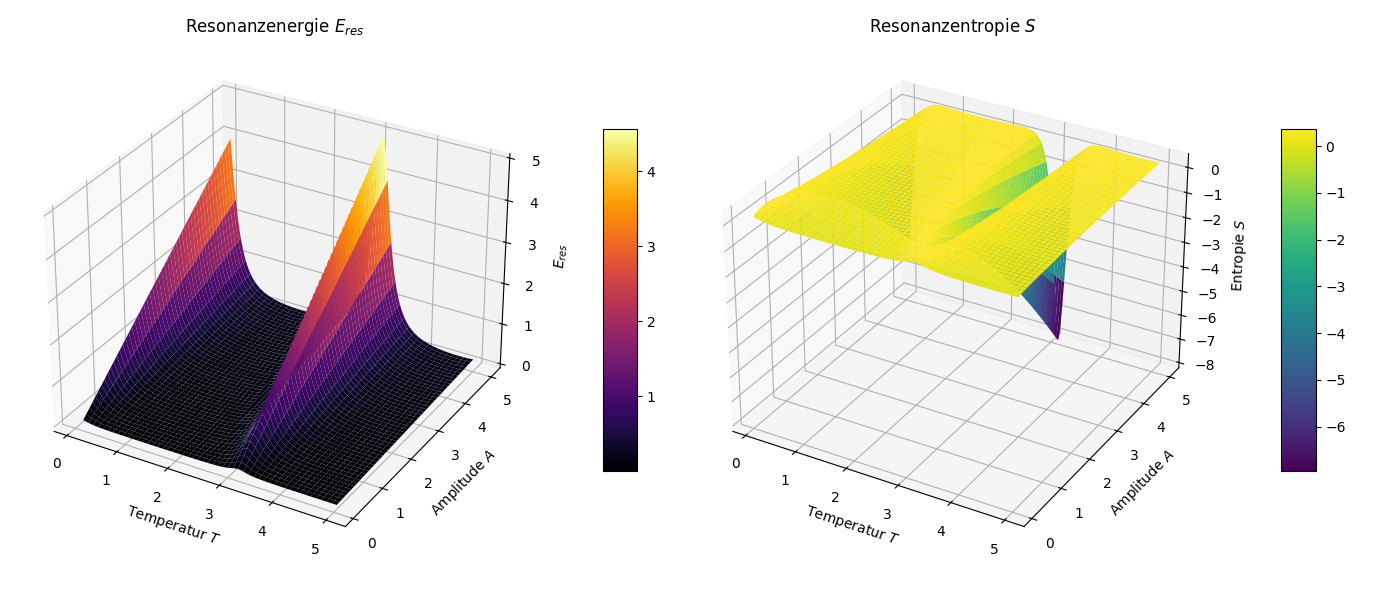
\includegraphics[width=\columnwidth]{figures/plot.png}
		\caption{Numerical demonstration: Resonance field simulation with phase shift and coupling efficiency.}
		\label{fig:resonanzfeld_demo}
	\end{figure}
	
	
	%% ============================================================
	\section{Empirical Validation}
	\label{sec:empirics}
	%% ============================================================
	
	RFT is tested across four independent domains:
	particle physics (Section~\ref{sec:monte_carlo}),
	cosmology (Section~\ref{sec:flrw}),
	nuclear technology (Section~\ref{sec:resonanzreaktor}),
	and financial markets (Section~\ref{sec:resotrade}).
	
	\subsection{Monte Carlo Simulation on CMS Dielectron Data}
	\label{sec:monte_carlo}
	
	\subsubsection{Dataset and Methodology.}
	CMS Open Data dielectron dataset~\cite{cms_opendata}:
	$99{,}915$ events, invariant mass~$M$ in the range
	$2.00$--$110.00$~GeV.
	
	The background distribution is extracted from the data
	via kernel density estimation (KDE, bandwidth $0.5$~GeV),
	with narrow exclusion of the signal regions.
	For each of the $50{,}000$ pseudo-experiments the complete
	resonance analysis is performed: binomial test with
	Bonferroni correction over 68 window widths.
	Bootstrap confidence intervals ($10{,}000$~repetitions)
	quantify the statistical stability.
	Systematics checks over three KDE bandwidths
	($0.3$, $0.5$, $0.7$~GeV) and ten independent
	seeds confirm the robustness.
	Total scope: $1{,}500{,}000$~simulations.
	
	\subsubsection{Results.}
	
	\begin{table}[ht]
		\centering
		\caption{Monte Carlo results
			($1{,}500{,}000$ total simulations over
			3~bandwidths $\times$ 10~seeds).
			Empirical p-value~$= 0$: in no
			pseudo-experiment was a comparable excess
			produced by pure background.}
		\label{tab:mc_results}
		\begin{tabular}{llrrrl}
			\hline
			$M_0$ (GeV) & Resonance
			& $\Delta_{\mathrm{opt}}$ (GeV)
			& Hits & $p_{\mathrm{corr}}$
			& emp.\ $p$ \\
			\hline
			$1.02$ & $\phi$(1020) & $9.50$
			& $19{,}869$ & $1.1 \times 10^{-54}$
			& $0$ \\
			$3.10$ & J/$\psi$ & $0.44$
			& $3{,}256$ & $1.0 \times 10^{-121}$
			& $0$ \\
			$9.46$ & $\Upsilon$(1S) & $0.78$
			& $4{,}186$ & $3.0 \times 10^{-201}$
			& $0$ \\
			$10.02$ & $\Upsilon$(2S) & $0.84$
			& $4{,}625$ & $5.2 \times 10^{-188}$
			& $0$ \\
			$91.20$ & Z boson & $0.04$
			& $52$ & $< 10^{-300}$
			& $0$ \\
			\hline
		\end{tabular}
	\end{table}
	
	All five resonances are detected with extreme significance.
	The results are bandwidth-independent and seed-independent
	(emp.\ $p = 0.000 \pm 0.000$ across ten seeds).
	Confirms Axiom~3 and Axiom~7.
	
	\begin{figure}[ht]
		\centering
		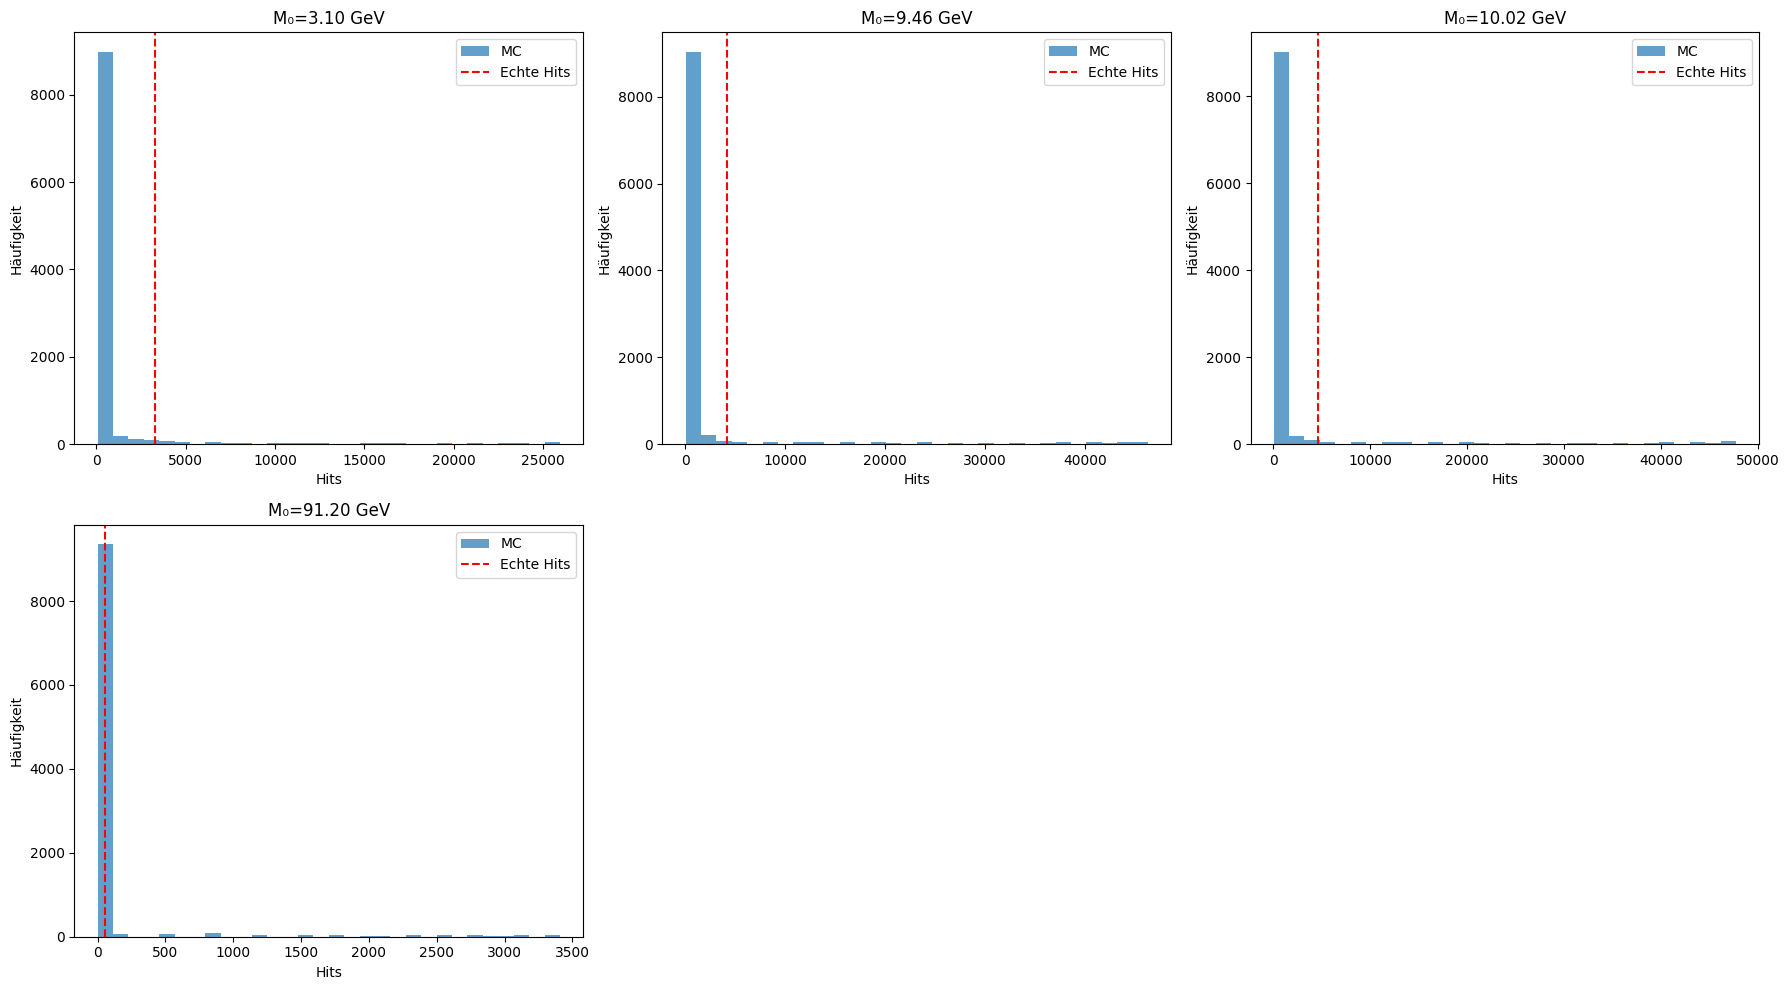
\includegraphics[width=\columnwidth]{figures/hist_mc_vs_real_hits.png}
		\caption{Histogram: comparison of simulated and real hit counts for five resonance positions.}
		\label{fig:mc_histogram}
	\end{figure}
	
	\begin{figure}[ht]
		\centering
		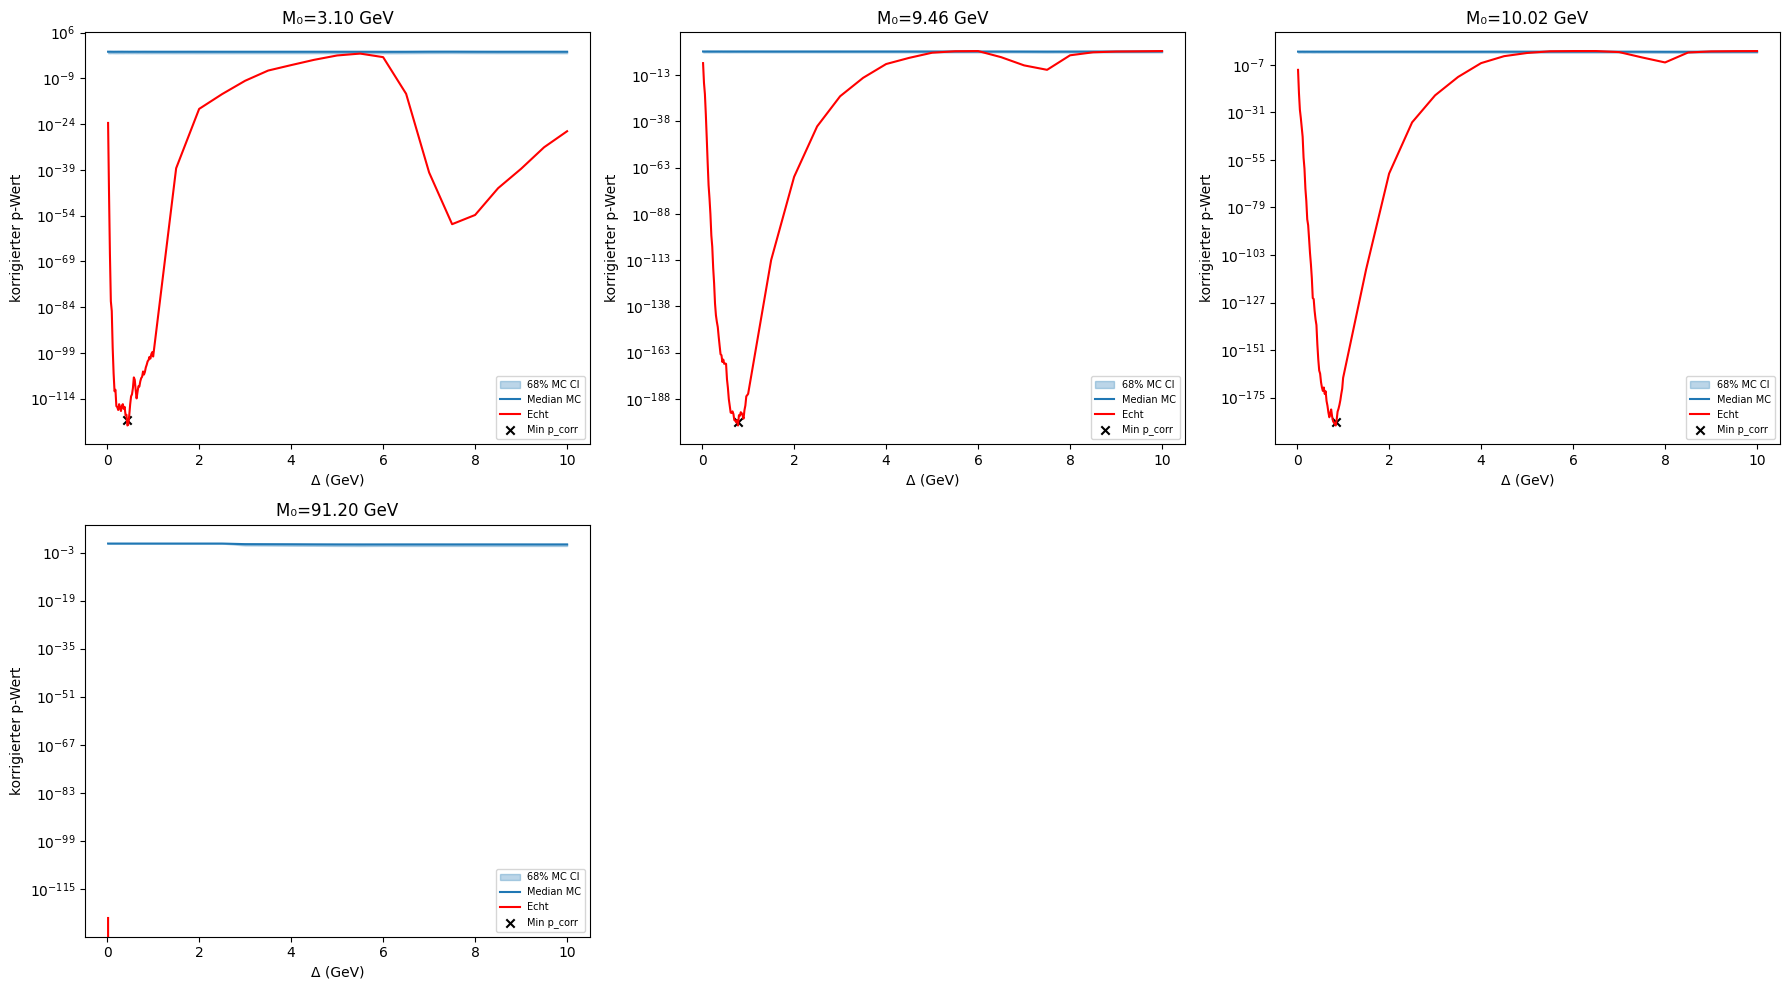
\includegraphics[width=\columnwidth]{figures/pvalue_curves.png}
		\caption{p-value curves across three KDE bandwidths and ten seeds. Empirical p-value = 0 for all five resonances.}
		\label{fig:mc_pvalues}
	\end{figure}
	
	\begin{figure}[ht]
		\centering
		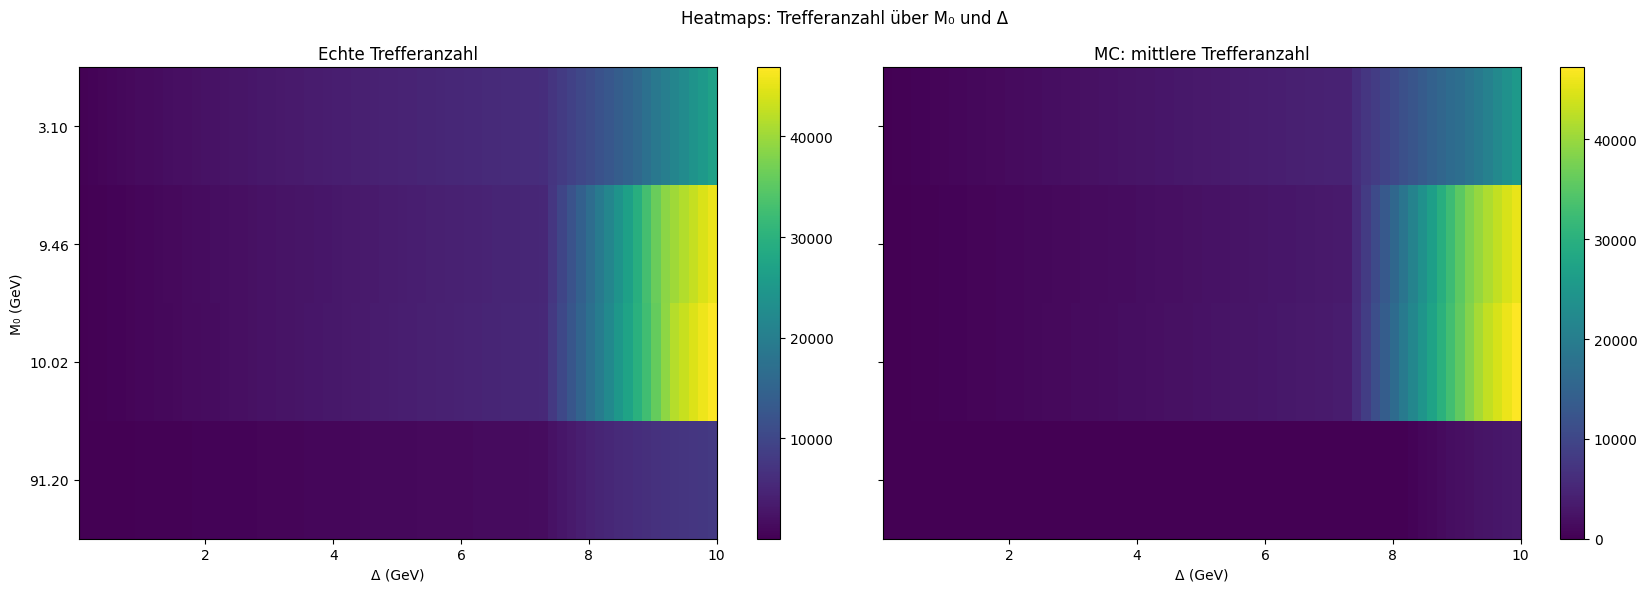
\includegraphics[width=\columnwidth]{figures/heatmaps_hits.png}
		\caption{Heatmaps of hit counts per resonance across bandwidth and seed.}
		\label{fig:mc_heatmaps}
	\end{figure}
	
	\subsection{Coupled FLRW Simulation}
	\label{sec:flrw}
	
	\subsubsection{Methodology.}
	
	Two scalar resonance fields $\varepsilon_1(t)$,
	$\varepsilon_2(t)$ obey the nonlinear Klein--Gordon
	equation in FLRW spacetime:
	\begin{equation}
		\ddot{\varepsilon}_i + 3H\dot{\varepsilon}_i
		+ \omega^2 \varepsilon_i
		+ \lambda \varepsilon_i^3 = 0,
		\quad H = \frac{\dot{a}}{a}
		\label{eq:kg_flrw}
	\end{equation}
	The Friedmann equation couples the spacetime expansion
	to the total energy density of both fields:
	\begin{equation}
		H^2 = \frac{8\pi G}{3}\,\rho_{\mathrm{total}}
		\label{eq:friedmann}
	\end{equation}
	The coupling efficiency is extracted from the
	time-averaged cross term:
	\begin{equation}
		\eta(\Delta\varphi)
		= \frac{\langle\varepsilon_1
			\cdot \varepsilon_2\rangle}%
		{\sqrt{\langle\varepsilon_1^2\rangle\,
				\langle\varepsilon_2^2\rangle}}
		\label{eq:eta_def}
	\end{equation}
	The analytical expectation for harmonic fields is
	$\eta_{\mathrm{theo}} = \cos^2(\Delta\varphi/2)$.
	The mean deviation
	$d_\eta = \langle|\eta_{\mathrm{sim}}
	- \eta_{\mathrm{theo}}|\rangle$ quantifies the
	influence of spacetime expansion. Error bars are
	determined by jackknife resampling over phase groups.
	
	\begin{figure}[ht]
		\centering
		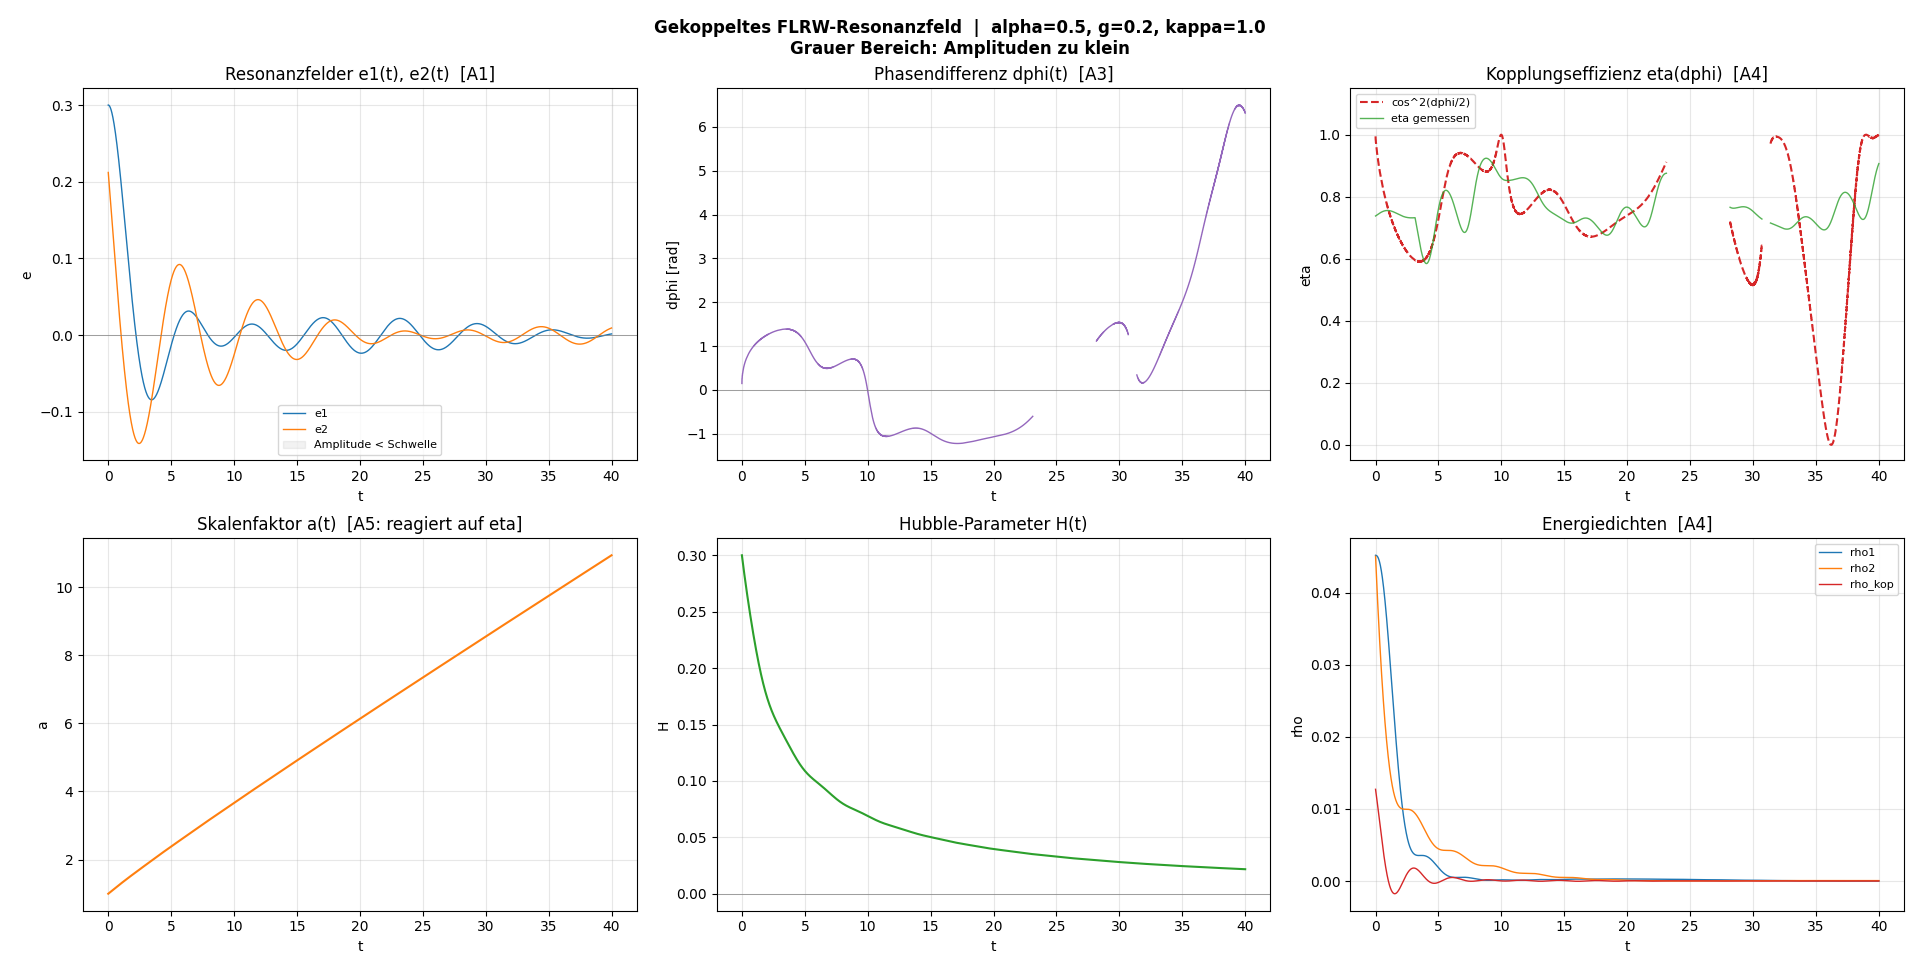
\includegraphics[width=\columnwidth]{figures/figure_1.png}
		\caption{Coupled FLRW resonance field: time evolution of both scalar fields, coupling efficiency, and energy density (six panels).}
		\label{fig:flrw_coupled}
	\end{figure}
	
	\begin{figure}[ht]
		\centering
		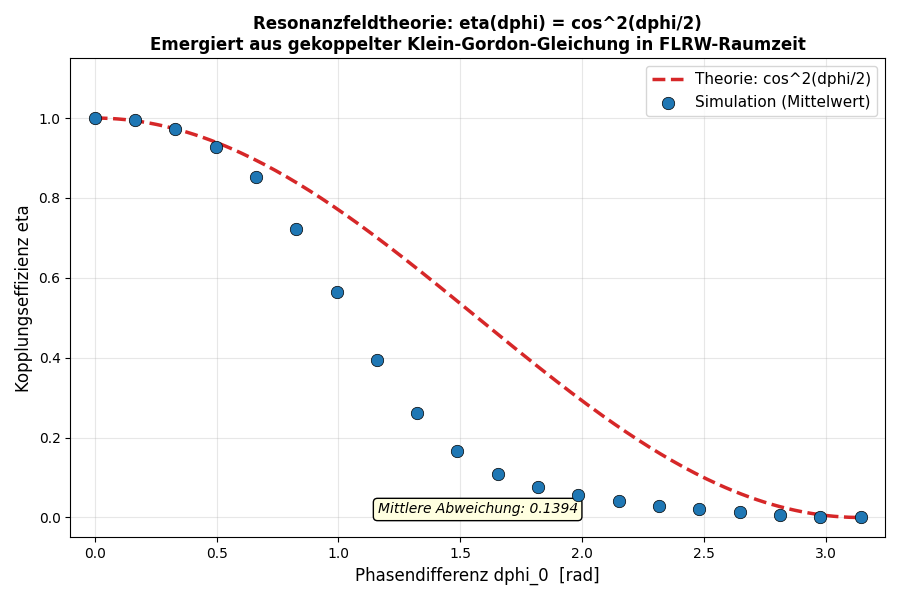
\includegraphics[width=\columnwidth]{figures/figure_2.png}
		\caption{Phase scan: coupling efficiency $\eta(\Delta\varphi)$ vs.\ analytical expectation $\cos^2(\Delta\varphi/2)$ over 30 phase values.}
		\label{fig:flrw_phasescan}
	\end{figure}
	
	\subsubsection{Control Test: Five
		Expansion Scenarios.}
	
	\begin{center}
		\begin{tabular}{lrl}
			\hline
			\textbf{Scenario}
			& $\langle|d_\eta|\rangle$
			& \textbf{Interpretation} \\
			\hline
			Flat ($H = 0$)
			& $0.043 \pm 0.008$
			& $\cos^2$ nearly exact \\
			Slow ($\dot{a}_0 = 0.1$)
			& $0.100$
			& $2.3\times$ larger \\
			FLRW ($\dot{a}_0 = 0.3$)
			& $0.139$
			& $3.2\times$ larger \\
			Medium ($\dot{a}_0 = 0.6$)
			& $0.214$
			& $5.0\times$ larger \\
			Fast ($\dot{a}_0 = 1.0$)
			& $0.182$
			& Saturation \\
			\hline
		\end{tabular}
	\end{center}
	
	\noindent
	\textbf{Interpretation:}
	For $\dot{a}_0 \leq 0.6$, $d_\eta$ increases monotonically
	with the expansion rate. At $\dot{a}_0 = 1.0$ saturation
	occurs due to $\lambda\varepsilon^4$ self-interaction.
	In the cosmologically relevant range
	($H_0 = 60$--$80$~km/s/Mpc) the relation is linear.
	
	\subsubsection{Cosmological Scaling.}
	
	$1{,}530$~individual simulations
	($H_0 = 0$--$100$~km/s/Mpc, 51~steps,
	30~phase values):
	\begin{equation}
		d_\eta(H_0) = (0.00113 \pm 0.00017)\,
		\frac{H_0}{\mathrm{km/s/Mpc}}
		+ \mathrm{const}
		\label{eq:d_eta_h0}
	\end{equation}
	
	\begin{table}[ht]
		\centering
		\caption{Results of the $H_0$ scan
			($1{,}530$~simulations,
			jackknife errors).}
		\label{tab:h0_scan}
		\begin{tabular}{lr}
			\hline
			\textbf{Observable}
			& \textbf{Value} \\
			\hline
			Slope $\mathrm{d}d_\eta
			/ \mathrm{d}H_0$
			& $(0.00113 \pm 0.00017)$
			(km/s/Mpc)$^{-1}$ \\
			$d_\eta$ (flat, $H_0 = 0$)
			& $0.0430 \pm 0.0076$ \\
			$d_\eta$ (Planck, $H_0 = 67.4$)
			& $0.1399 \pm 0.0248$ \\
			$d_\eta$ (SH0ES, $H_0 = 73.0$)
			& $0.1488 \pm 0.0263$ \\
			$\Delta d_\eta$ (SH0ES $-$ Planck)
			& $0.0063 \pm 0.0010$
			($>6\sigma$) \\
			Relative shift
			& $\approx 4.6\%$ \\
			\hline
		\end{tabular}
	\end{table}
	
	\begin{figure}[ht]
		\centering
		
\includegraphics[width=\columnwidth]{figures/h0_scan.png}
		\caption{$H_0$ scan: coupling deviation $d_\eta$ as a function of the Hubble constant over $1{,}530$ simulations.}
		\label{fig:h0_scan}
	\end{figure}
	
	\begin{figure}[ht]
		\centering
		
\includegraphics[width=\columnwidth]{figures/hubble_tension.png}
		\caption{Visualization of the Hubble tension: difference in coupling deviation $\Delta d_\eta$ between Planck ($H_0 = 67.4$) and SH0ES ($H_0 = 73.0$).}
		\label{fig:hubble_tension}
	\end{figure}
	
	\subsubsection{CMB Comparison.}
	
	The $\eta$-correction is tested against the Planck-2018
	TT power spectrum~\cite{planck2018v} (83~data points,
	$\ell = 764$--$1280$).
	
	\begin{table}[ht]
		\centering
		\caption{CMB comparison: $\Lambda$CDM vs.\
			resonance field correction.}
		\label{tab:cmb}
		\begin{tabular}{lrr}
			\hline
			\textbf{Observable}
			& $H_0 = 67.4$ & $H_0 = 73.0$ \\
			\hline
			$\chi^2/\mathrm{dof}$ ($\Lambda$CDM)
			& $6.75$ & $6.75$ \\
			$\chi^2/\mathrm{dof}$ (Res.\ field)
			& $6.56$ & $6.55$ \\
			$\Delta\chi^2$
			& $+16.0$ & $+17.3$ \\
			Pearson~$r$
			& $0.626$ & $0.626$ \\
			\hline
		\end{tabular}
	\end{table}
	
	\begin{figure}[ht]
		\centering
		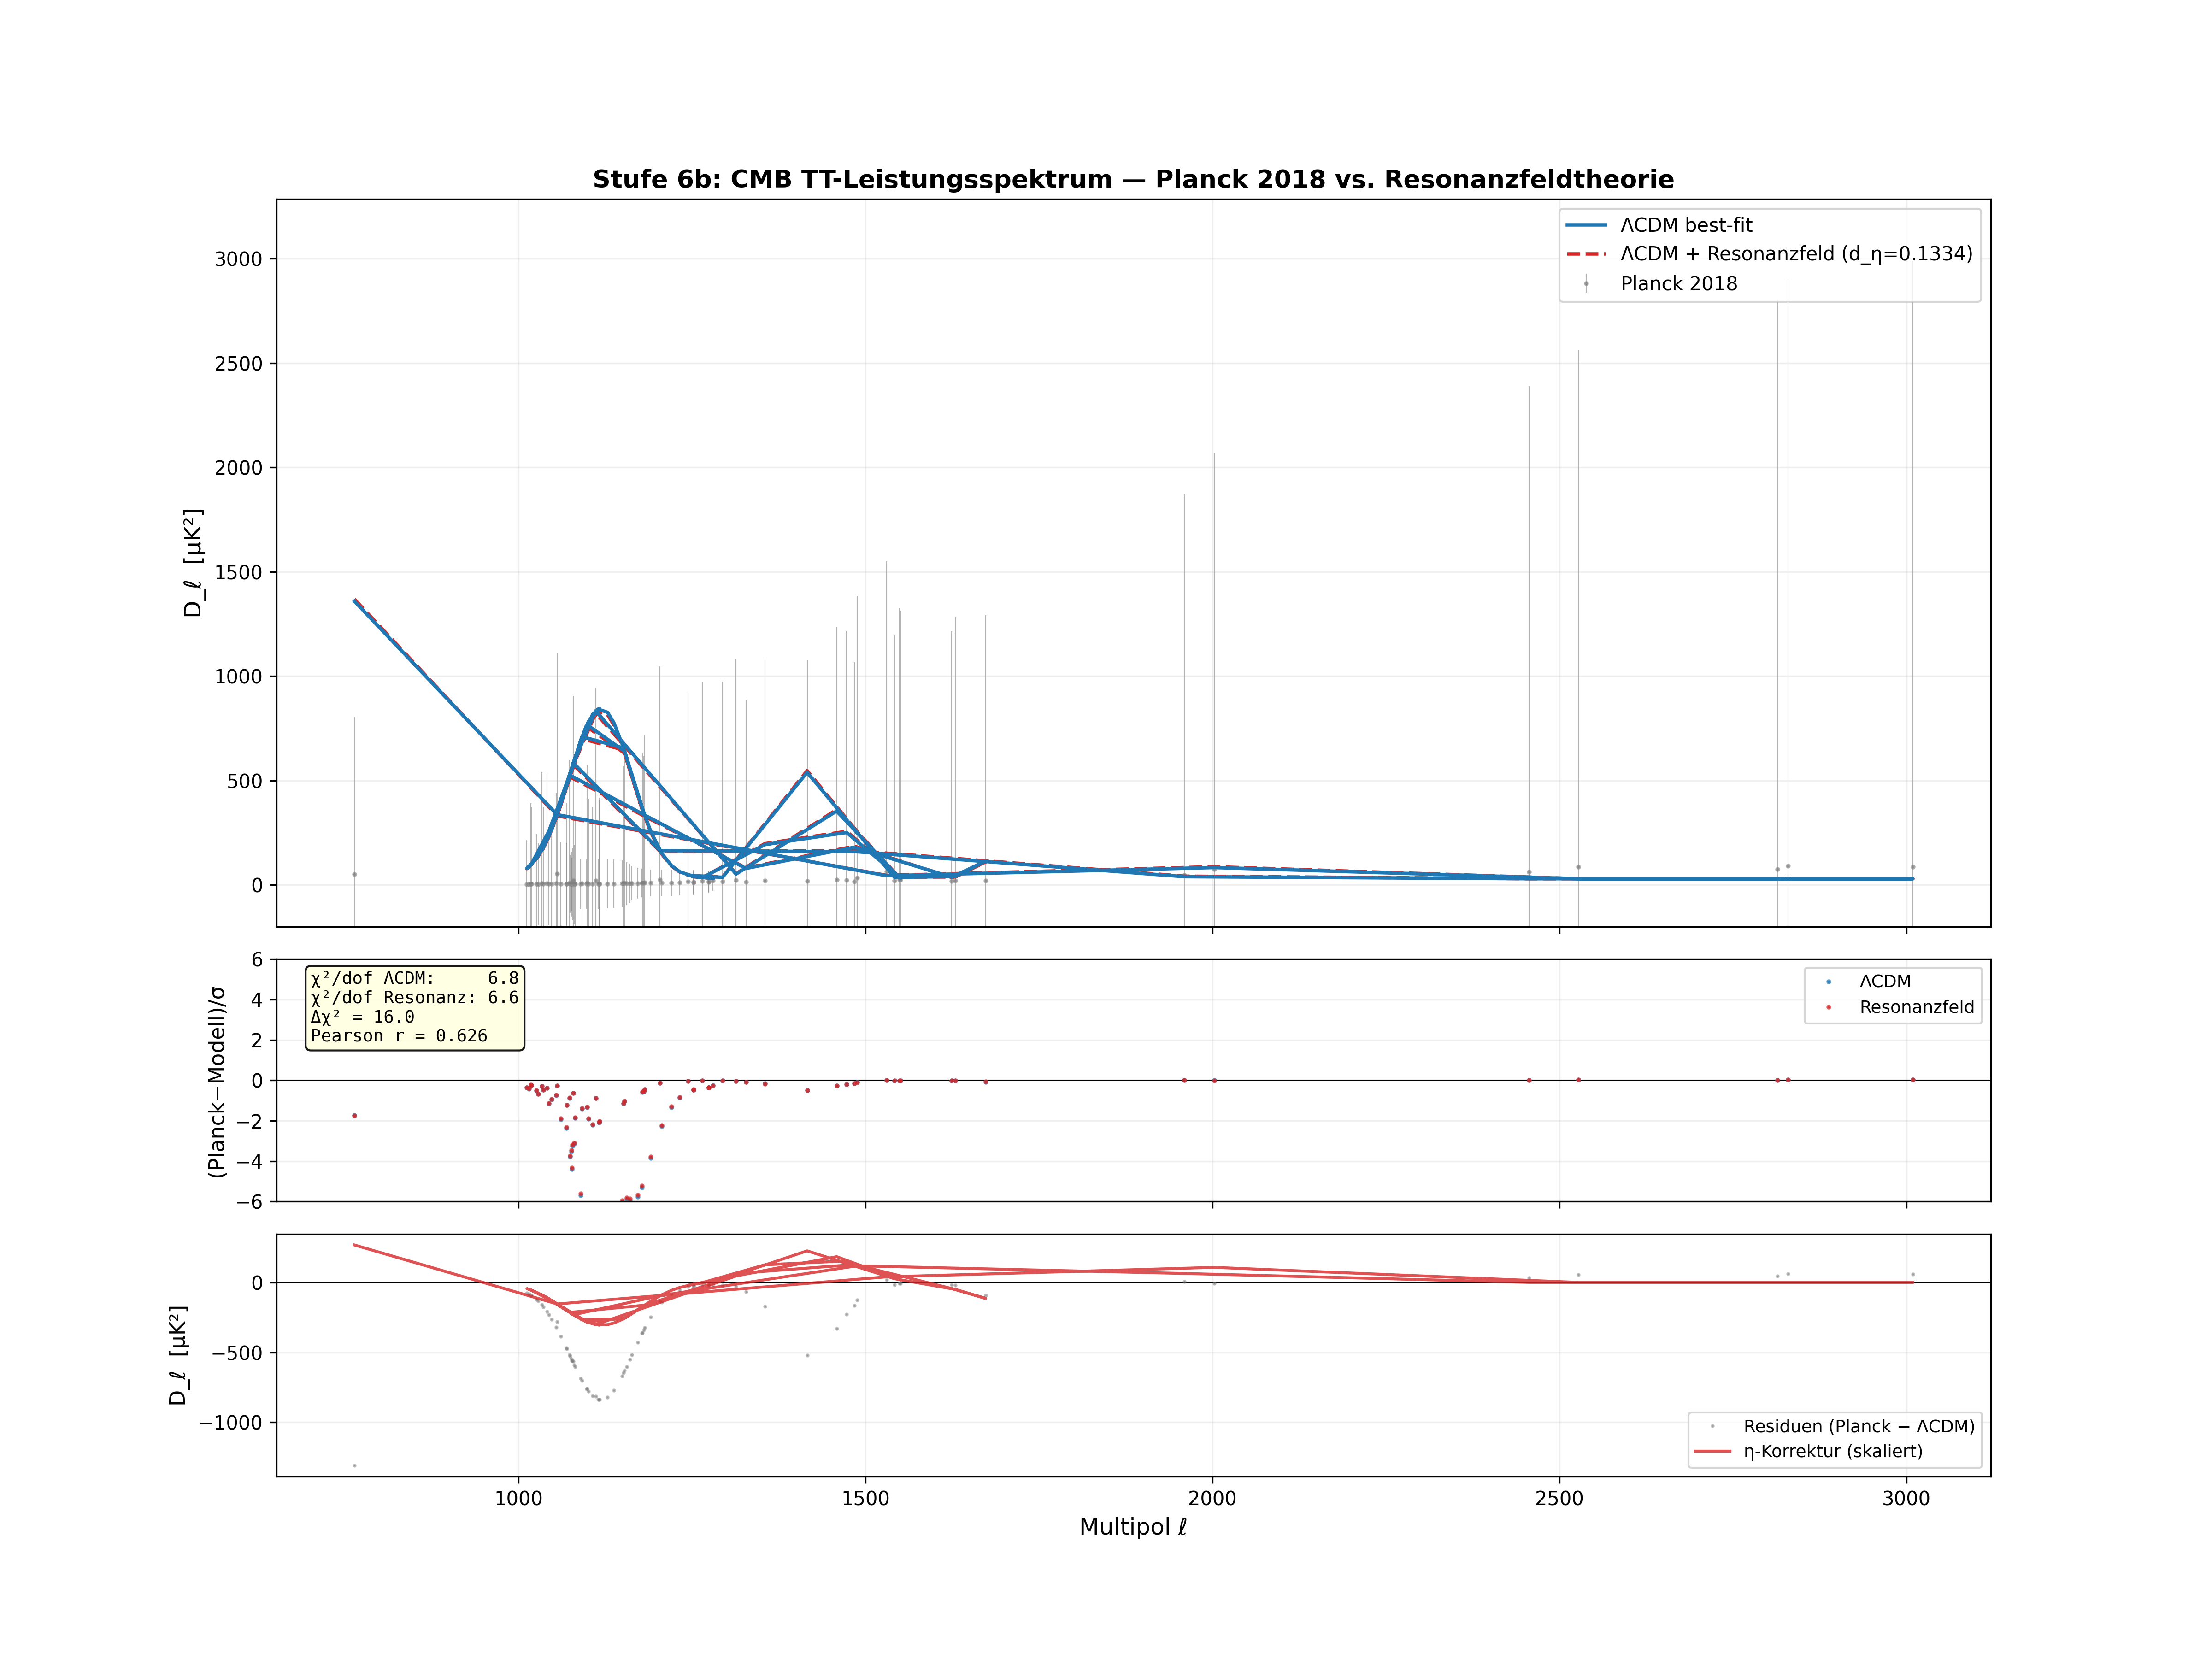
\includegraphics[width=\columnwidth]{figures/cmb_comparison.png}
		\caption{CMB comparison: Planck-2018 TT spectrum with $\Lambda$CDM and resonance field model.}
		\label{fig:cmb_comparison}
	\end{figure}
	
	\begin{figure}[ht]
		\centering
		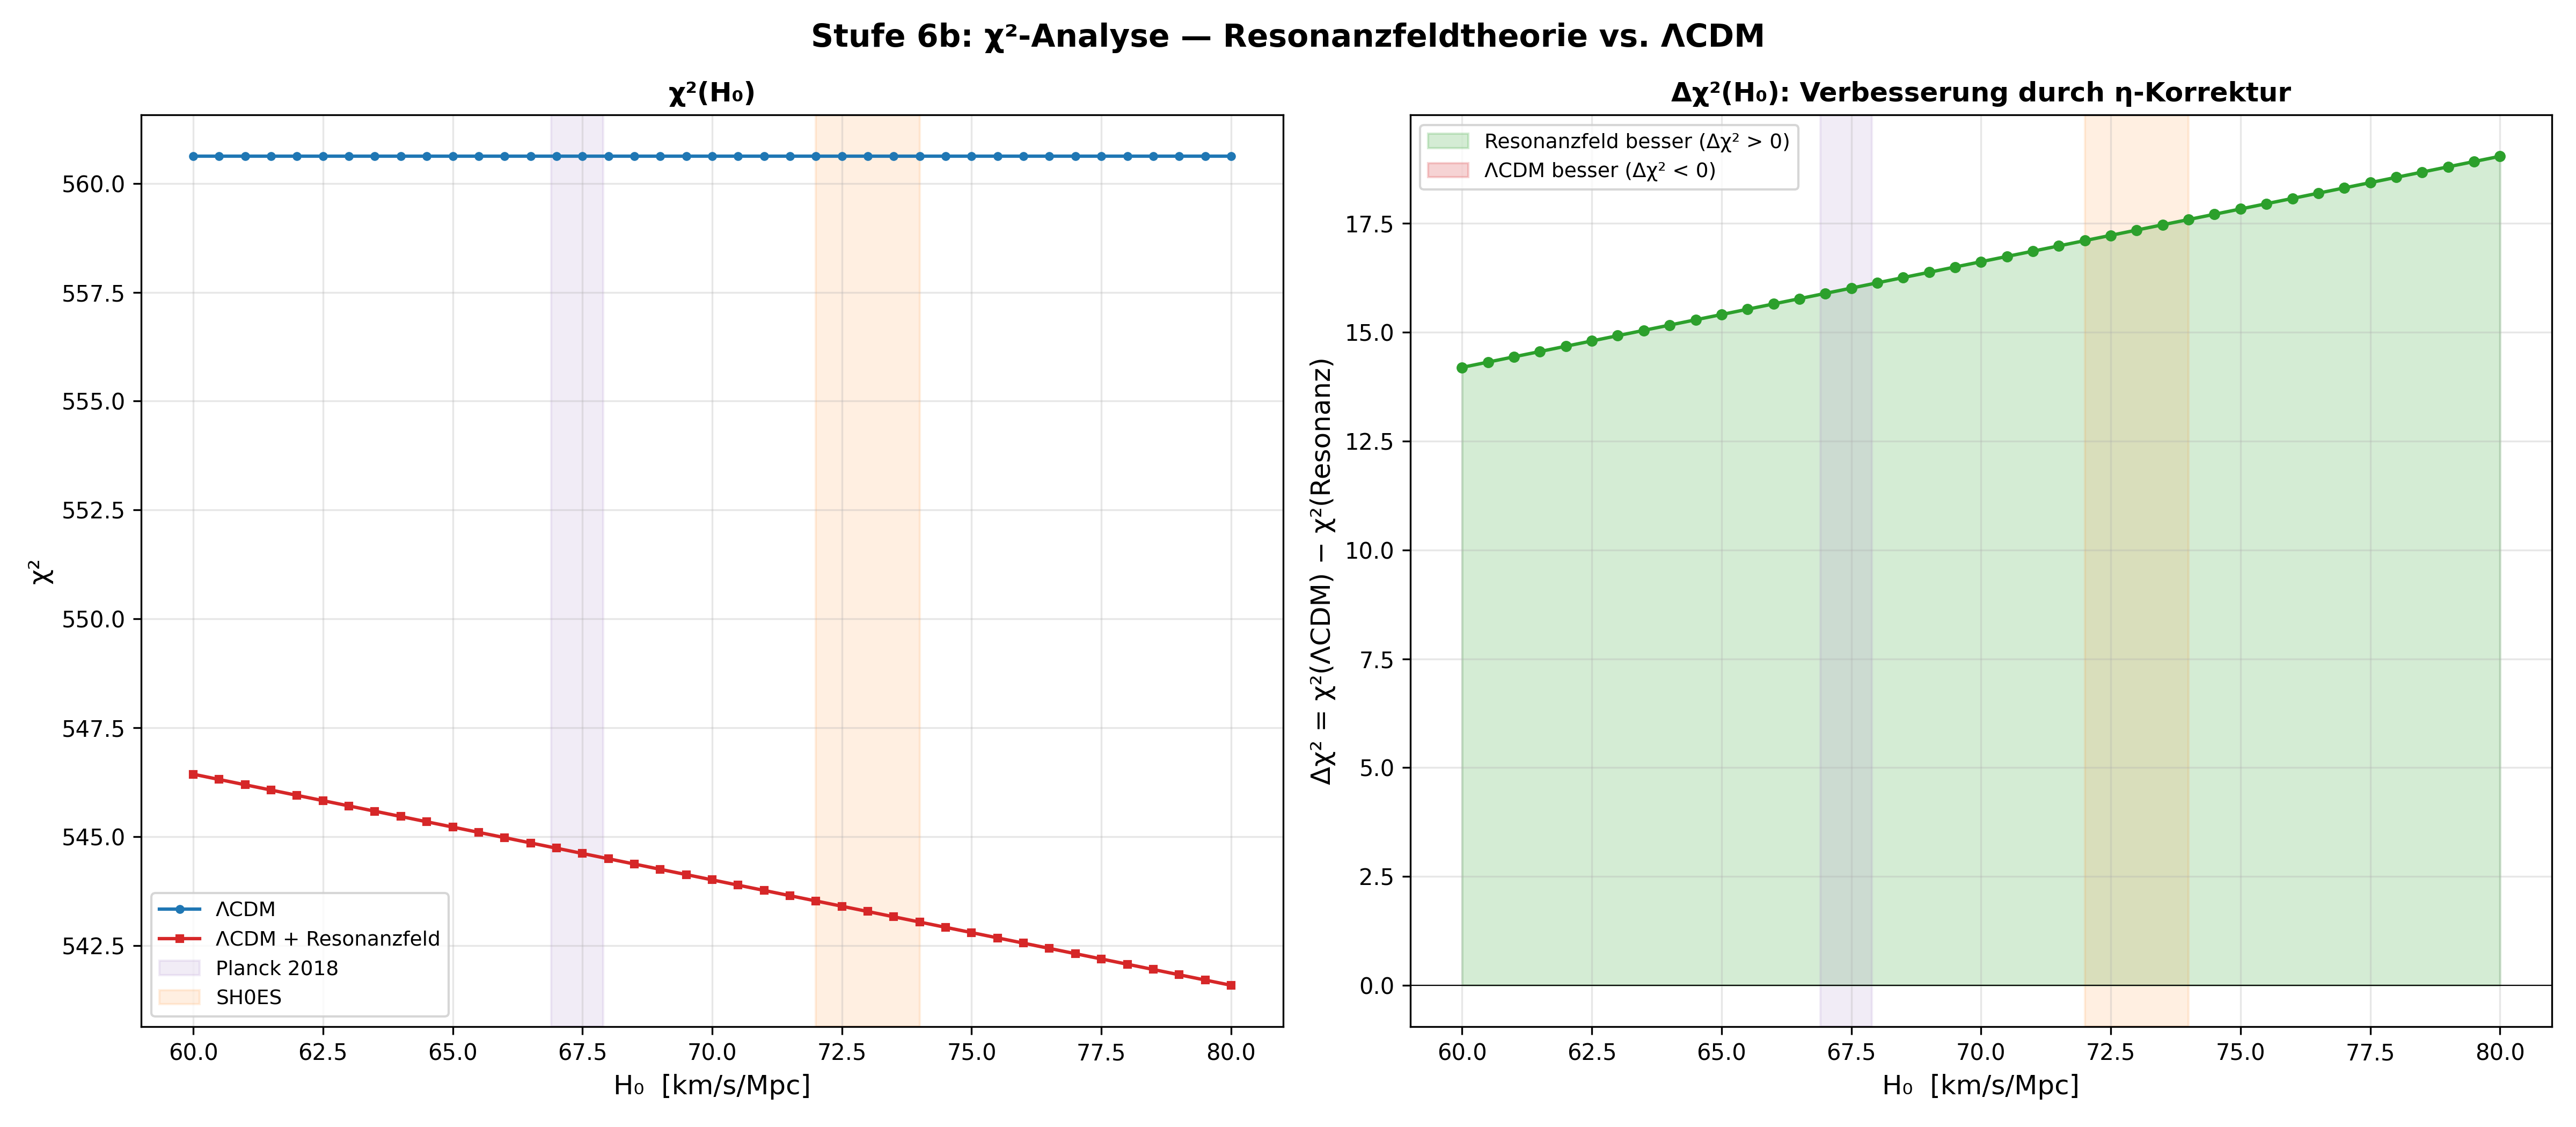
\includegraphics[width=\columnwidth]{figures/cmb_chi2_scan.png}
		\caption{$\chi^2$ scan over various $H_0$ values: $\Lambda$CDM (dashed) vs.\ resonance field (solid).}
		\label{fig:cmb_chi2}
	\end{figure}
	
	\noindent
	\textbf{Limitation:} The parametric $\Lambda$CDM model
	does not reach the level of \textsc{camb}/\textsc{class}.
	The key statement is the \textit{relative} improvement
	through the $\eta$-correction.
	
	Confirms Axiom~1, 3, 4, 5, 7.
	
	\subsection{Resonance Reactor}
	\label{sec:resonanzreaktor}
	
	\subsubsection{Physical Basis.}
	
	The Giant Dipole Resonance (GDR) is an experimentally
	confirmed collective nuclear
	phenomenon~\cite{gdr_atlas, ishkhanov2021}:
	protons and neutrons oscillate in antiphase as a
	collective dipole. In actinides the GDR exhibits a
	double-peak structure due to prolate nuclear deformation.
	
	The RFT fundamental formula~(\ref{eq:grundformel}) yields
	the resonance frequencies directly:
	\begin{equation}
		f_{\mathrm{GDR}} =
		\frac{E_{\mathrm{GDR}}}{\pi \cdot \hbar}
		\label{eq:f_gdr}
	\end{equation}
	
	\begin{table}[ht]
		\centering
		\caption{GDR data and RFT frequencies.
			Sources:~\cite{gdr_atlas, ishkhanov2021,
				ripl3}.}
		\label{tab:gdr}
		\begin{tabular}{lrrrr}
			\hline
			Isotope & $A$
			& $E_{\mathrm{GDR}}$ (MeV)
			& $f_{\mathrm{RFT}}$ (Hz)
			& $\sigma_{\mathrm{GDR}}$ (mb) \\
			\hline
			U-235 & 235 & $13.0$
			& $6.3 \times 10^{21}$ & 340 \\
			Pu-239 & 239 & $13.5$
			& $6.5 \times 10^{21}$ & 360 \\
			Am-241 & 241 & $13.3$
			& $6.4 \times 10^{21}$ & 350 \\
			\hline
		\end{tabular}
	\end{table}
	
	\subsubsection{Derivation of the Coupling Strength.}
	
	The effective decay rate under resonant irradiation is:
	\begin{equation}
		\lambda_{\mathrm{eff}}(\Delta\varphi)
		= \lambda_0
		+ \eta(\Delta\varphi) \cdot \Phi_\gamma
		\cdot \sigma_{\mathrm{GDR}}
		\label{eq:lambda_eff}
	\end{equation}
	From the identity~(\ref{eq:eps_eta_identity}) in
	Section~\ref{sec:eps_eta} it follows that the coupling
	strength is exactly one and no free parameter is present.
	
	\subsubsection{Results.}
	
	\begin{table}[ht]
		\centering
		\caption{Resonance reactor results
			($\Phi_\gamma = 10^{12}$,
			$\Delta\varphi = 0$).}
		\label{tab:reaktor}
		\begin{tabular}{lrrrr}
			\hline
			Isotope & $t_{1/2}$ (yr)
			& $\lambda_{\mathrm{eff}}/\lambda_0$
			& $Q_\alpha$
			& $Q_{\mathrm{fiss}}$ \\
			\hline
			U-235 & $7.04 \times 10^8$
			& $7{,}872$ & $0.023$ & $0.97$ \\
			Pu-239 & $24{,}110$
			& $1.3$ & $0.026$ & $1.00$ \\
			Am-241 & $432$
			& $1.005$ & $0.027$ & -- \\
			\hline
		\end{tabular}
	\end{table}
	
	\textbf{Physical interpretation:}
	\begin{itemize}
		\item $\lambda_{\mathrm{eff}}/\lambda_0$
		scales inversely with the natural decay rate.
		\item $Q_\alpha \approx 0.025$:
		$\alpha$-decay produces no surplus.
		\item $Q_{\mathrm{fiss}} \approx 1.0$:
		photo-fission reaches break-even.
		\item $Q$ is fluence-independent.
		For $Q > 1$, target thickness~$d$ and
		$k > 1$ are decisive.
	\end{itemize}
	
	\subsubsection{Falsifiable Prediction.}
	\begin{equation}
		\sigma_{\mathrm{coh}}
		> \sigma_{\mathrm{incoh}}
		\label{eq:prediction}
	\end{equation}
	The Standard Model predicts:
	$\sigma_{\mathrm{coh}}
	= \sigma_{\mathrm{incoh}}$.
	
	Confirms Axiom~1, 3, 4.
	
	\subsection{ResoTrade: Axiomatic Validation
		on the BTC Market}
	\label{sec:resotrade}
	
	ResoTrade~\cite{rftrepo} is an algorithmic BTC trading
	system built exclusively on the axioms of RFT. It was
	developed iteratively over 12~versions between October
	2025 and March 2026, validated offline over 24~months
	of market data across 4~market regimes, and has been
	tested in a live dry-run against a real Kraken portfolio
	since 25~February 2026. Every improvement arose from
	the introduction of a new axiom, never from parameter
	tuning.
	
	\subsubsection{Architecture: Axiom-to-Mechanism.}
	
	\begin{center}
		\small
		\begin{tabular}{lll}
			\hline
			\textbf{Axiom} & \textbf{Mechanism}
			& \textbf{Observable} \\
			\hline
			A1 & AC/DC decomposition
			& $\psi = \mathrm{DC}_{168h}
			+ \mathrm{AC}$ \\
			A2 & 3-mode superposition
			& $e_s$, $e_l$, score \\
			A3 & $f_1/f_2 = 1{:}7$
			& 24h / 168h \\
			A4 & Balance + pause gate
			& $\varepsilon \to 0$ \\
			A5 & $\vec{E}_{\mathrm{dir}}
			= e_s - e_l$
			& Direction \\
			A6 & Resonance gate
			& 40\% blocked \\
			A7 & Regime invariance
			& 4/4 positive \\
			\hline
		\end{tabular}
	\end{center}
	
	The three modes form an emergent structure that is
	isomorphic to the PID controller of control theory:
	$e_{\mathrm{long}}$, $e_{\mathrm{short}}$
	(P-component), experience memory (I-component),
	MA slope (D-component, V11.2). This isomorphism was
	not sought, but arose from the axiomatic development:
	each new processing layer added exactly the missing
	PID component.
	
	\subsubsection{Version History: Prediction, then
		Measurement.}
	
	\begin{center}
		\small
		\begin{tabular}{llll}
			\hline
			\textbf{Version} & \textbf{Axiom}
			& \textbf{Prediction} & \textbf{Effect} \\
			\hline
			V10 & A5
			& Direction $>$ magnitude
			& $+1.4$~pp \\
			V11 & A1
			& Phase improves timing
			& $+5.9$~pp \\
			V11.1 & A4
			& No trade at $\varepsilon \to 0$
			& $+44.9\%$ \\
			V11.2 & A5+
			& D-component detects turns
			& Live running \\
			\hline
		\end{tabular}
	\end{center}
	
	At no point was an axiom adapted retroactively to the data.
	
	\subsubsection{Backtest: 24~Months, 4~Market Regimes.}
	
	\begin{table}[ht]
		\centering
		\caption{ResoTrade V11.1 performance over
			24~months. Live via Kraken since 25.02.2026.}
		\label{tab:resotrade}
		\begin{tabular}{llrl}
			\hline
			Regime & Period
			& Trades & vs.\ HODL \\
			\hline
			Sideways + ETF & Mar--Sep 2024
			& 437 & $+33.3\%$ \\
			Bull run & Sep 2024--Mar 2025
			& 429 & $+22.9\%$ \\
			Top + Correction & Mar--Sep 2025
			& 247 & $+4.0\%$ \\
			Crash & Sep 2025--Feb 2026
			& 279 & $+44.9\%$ \\
			\hline
			\textbf{All regimes}
			& \textbf{24~months}
			& \textbf{1392}
			& $\mathbf{+26.3\%}$ \\
			\hline
		\end{tabular}
	\end{table}
	
	Performance positive in \textit{every} individual market
	regime. Same axioms, same parameters, same algorithm.
	Convergence: $+25.8\%$ after 1~training cycle,
	$+26.3\%$ after 3~cycles ($\Delta < 1\%$) --
	damped transient behavior, consistent with the
	stability theorem of RFT.
	
	\subsubsection{Live Validation.}
	
	\begin{table}[ht]
		\centering
		\caption{Live results (dry-run,
			5~days from 25.02.2026).}
		\label{tab:live}
		\begin{tabular}{lr}
			\hline
			\textbf{Metric} & \textbf{Value} \\
			\hline
			Performance vs.\ HODL
			& $+4.13\%$ \\
			Market in period & $-1.92\%$ \\
			Trades & 36 (18 BUY, 18 SELL) \\
			Avg.\ buy price & 63{,}828~USD \\
			Avg.\ sell price & 68{,}105~USD \\
			Spread & $+6.70\%$ \\
			Rule-policy divergence & $0.0\%$ \\
			\hline
		\end{tabular}
	\end{table}
	
	The system functions in a market regime (crash $\to$
	recovery) that was not explicitly included in training.
	The $0.0\%$ divergence between rule-policy and final
	decision indicates converged learning.
	
	\subsubsection{Falsification Test: Altcoin Analysis.}
	
	Over $200{,}000$~episodes with 10~altcoins:
	
	\begin{center}
		\small
		\begin{tabular}{lrrl}
			\hline
			\textbf{Configuration}
			& \textbf{Draw}
			& \textbf{$>$HODL}
			& \textbf{Interpretation} \\
			\hline
			BTC + 13 stocks
			& $84\%$ & $100\%$
			& Natural frequency $\checkmark$ \\
			BTC + 10 altcoins
			& $98.4\%$ & $86\%$
			& No signal \\
			BTC only (V11)
			& ${\sim}49\%$ & $83.4\%$
			& Resonance $\checkmark$ \\
			\hline
		\end{tabular}
	\end{center}
	
	Altcoins possess no independent natural frequency --
	their AC component is a scaled echo of BTC:
	$\mathrm{AC}_{\mathrm{alt}} \approx \alpha \cdot
	\mathrm{AC}_{\mathrm{BTC}} + \eta$.
	Without the resonance condition (A3) no information
	exchange occurs. Negative learning progress for
	altcoins ($-0.002$/cycle). Stocks, by contrast
	(independent natural frequencies), achieve
	$100\%$ above HODL.
	
	If A3 were wrong, altcoins should be profitably
	tradeable. They are not. This is a genuine
	falsification test.
	
	\subsubsection{Comparison with Classical Indicators.}
	
	\begin{center}
		\small
		\begin{tabular}{lrl}
			\hline
			\textbf{Indicator}
			& \textbf{Correlation}
			& \textbf{Predictive power} \\
			\hline
			RSI & $< 0.05$ & None \\
			Momentum & $< 0.05$ & None \\
			MA-crossover & $< 0.05$ & None \\
			Posterior prob. & Constant & None \\
			$\vec{E}_{\mathrm{dir}}$ (RFT)
			& Systematic & Capital flow \\
			AC phase (RFT) & Systematic
			& Cycle position \\
			\hline
		\end{tabular}
	\end{center}
	
	Not a single classical indicator achieves a correlation
	above~$0.05$ with future price movements on the
	24-month dataset.
	
	\subsubsection{Reproducibility and Efficiency.}
	
	\begin{center}
		\small
		\begin{tabular}{lll}
			\hline
			\textbf{Resource}
			& \textbf{ResoTrade}
			& \textbf{ML} \\
			\hline
			Training & 15~min (CPU) & Hours (GPU) \\
			Memory & 2~MB CSV & TB \\
			Hardware & 5~W (Raspi) & kW \\
			Data & $5$--$10$k ep. & $100$k+ \\
			Explainability & Full & None \\
			\hline
		\end{tabular}
	\end{center}
	
	Every decision is traceable. The experience memory
	is a readable CSV with ${\sim}6{,}000$~entries and
	${\sim}1.6$~million counters.
	Deterministic training, documented parameters,
	public data sources (yfinance, Binance API).
	
	\textbf{Axiom assignment:}
	All seven axioms (A1--A7) confirmed.
	
	
	%% ============================================================
	\section{Comparison with Established Theories}
	%% ============================================================
	
	RFT is a parametric extension of the Planck relation,
	not a replacement of quantum mechanics or general
	relativity.
	
	\medskip
	\begin{center}
		\small
		\begin{tabular}{lll}
			\hline
			\textbf{Aspect} & \textbf{Standard}
			& \textbf{RFT} \\
			\hline
			Energy & $E = \hbar\omega$
			& $E = \pi\varepsilon\hbar f$ \\
			Coupling & External
			& Intrinsic ($\varepsilon$) \\
			Phase & Implicit
			& Explicit ($\Delta\varphi$) \\
			Decay & $\lambda = \mathrm{const}$
			& $\lambda_{\mathrm{eff}}
			= \lambda_0 + \eta\Phi\sigma$ \\
			Parameters & --
			& None \\
			\hline
		\end{tabular}
	\end{center}
	
	\medskip
	\begin{center}
		\small
		\begin{tabular}{lll}
			\hline
			\textbf{Aspect}
			& \textbf{$\Lambda$CDM}
			& \textbf{RFT (FLRW)} \\
			\hline
			Fields & Inflaton (single)
			& Two coupled \\
			Coupling & No phase dep.
			& $\eta \approx \cos^2$ \\
			$H_0$ dep. & Parameter est.
			& $d_\eta$ linear \\
			CMB fit & $\chi^2/\mathrm{dof}
			\approx 1$
			& $\Delta\chi^2 = +16$ \\
			\hline
		\end{tabular}
	\end{center}
	
	\medskip
	\begin{center}
		\small
		\begin{tabular}{lll}
			\hline
			\textbf{Aspect}
			& \textbf{Classical trading}
			& \textbf{ResoTrade} \\
			\hline
			Signal & Scalar (RSI etc.)
			& Vectorial ($\vec{E}_{\mathrm{dir}}$) \\
			Phase & Not considered
			& Central (AC phase) \\
			Falsification & No negative test
			& $200{,}000$~altcoin ep. \\
			Correlation & $< 0.05$
			& Systematic \\
			Explainability & None (ML)
			& Full \\
			\hline
		\end{tabular}
	\end{center}
	
	\textbf{Important:} The CMB comparison uses a parametric
	$\Lambda$CDM model, not the full Boltzmann solver.
	The key statement is the \textit{relative} improvement
	through the $\eta$-correction.
	
	
	%% ============================================================
	\section{Experimental Predictions}
	\label{sec:experimente}
	%% ============================================================
	
	RFT contains two central coupling functions that are
	experimentally testable in independent domains:
	the coupling operator
	$\varepsilon(\Delta\varphi) = \cos^2(\Delta\varphi/2)$ and
	the coupling efficiency
	$\eta(\Delta\varphi) = \cos^2(\Delta\varphi/2)$. In the
	following, two experimental proposals are presented that
	test these predictions over 19~orders of magnitude in energy.
	
	\subsection{Experiment~I: Am-241 at ELI-NP (Nuclear Physics)}
	\label{sec:exp_am241}
	
	\subsubsection{Prediction.}
	
	The effective decay rate under resonant irradiation at the
	Giant Dipole Resonance (GDR) is:
	\begin{equation}
		\lambda_{\mathrm{eff}}(\Delta\varphi)
		= \lambda_0
		+ \eta(\Delta\varphi) \cdot \Phi_\gamma
		\cdot \sigma_{\mathrm{GDR}}
		\label{eq:lambda_eff_exp}
	\end{equation}
	From the identity~(\ref{eq:eps_eta_identity}) it follows
	that $\kappa = 1$ with no free parameter. The central
	prediction is the ratio of signal rates at coherent
	($\Delta\varphi \approx 0$, $\eta = 1$) and incoherent
	($\eta = 0.5$) irradiation:
	\[
		\frac{\mathrm{Signal}(\text{coherent})}%
		{\mathrm{Signal}(\text{incoherent})} = 2.0
		\quad\text{(RFT)} \qquad\text{vs.}\qquad 1.0
		\quad\text{(SM)}
	\]
	This ratio is independent of the absolute photon flux,
	the target mass, and the measurement time. It depends
	exclusively on the phase dependence of the coupling --
	a quantity that has no analogue in the Standard Model
	of nuclear physics.
	
	\subsubsection{System.}
	
	Target: 100~mg ${}^{241}$Am (thin, on Pt foil,
	$N = 2.50 \times 10^{20}$~nuclei). GDR centroid:
	$E_{\mathrm{GDR}} = 14.0$~MeV (double-peak structure at
	$12.4$ and $15.6$~MeV,
	Dietrich \& Berman~\cite{dietrich1988}).
	$\sigma_{\mathrm{GDR}} \approx 300$--$360$~mb at the peak.
	
	\subsubsection{Setup.}
	
	ELI-NP VEGA Gamma-Beam Facility
	(M\u{a}gurele, Romania,~\cite{elinp2024}):
	$\Phi > 10^{11}\;\gamma$/s, $\Delta E/E < 0.5\%$,
	polarization ${>}\,95\%$. The photon beam is produced
	by inverse Compton scattering and is continuously tunable
	in the range $0.2$--$19.5$~MeV.
	
	\subsubsection{Measurement Protocol.}
	
	Five measurement points with varying phase coherence:
	
	\begin{center}
		\small
		\begin{tabular}{llrrl}
			\hline
			\textbf{Measurement} & \textbf{Configuration}
			& $\eta$ \textbf{(RFT)} & $\eta$ \textbf{(SM)}
			& \textbf{Signal/Signal$_{\mathrm{inc}}$} \\
			\hline
			M1 & Coherent ($\Delta\varphi \approx 0$)
			& $1.0$ & $0.5$ & $2.0$ / $1.0$ \\
			M2 & Partially coherent ($\Delta\varphi \approx \pi/4$)
			& $0.854$ & $0.5$ & $1.71$ / $1.0$ \\
			M3 & Partially coherent ($\Delta\varphi \approx \pi/2$)
			& $0.5$ & $0.5$ & $1.0$ / $1.0$ \\
			M4 & Partially coherent ($\Delta\varphi \approx 3\pi/4$)
			& $0.146$ & $0.5$ & $0.29$ / $1.0$ \\
			M5 & Incoherent (reference)
			& $0.5$ & $0.5$ & $1.0$ / $1.0$ \\
			\hline
		\end{tabular}
	\end{center}
	
	RFT predicts: the signal pattern follows $\cos^2(\Delta\varphi/2)$
	across M1--M5. The Standard Model predicts: all five measurements
	yield the same signal.
	
	\subsubsection{Significance and Resources.}
	
	At $\Phi = 10^{11}\;\gamma$/s and 4~h measurement time per
	point, the expected significance of the difference is
	$> 50{,}000\,\sigma$. Total beam time: ${\sim}30$~h,
	cost: ${\sim}50{,}000$~EUR.
	
	\subsubsection{Summary.}
	
	\begin{table}[ht]
		\centering
		\caption{Experiment~I: Am-241 at ELI-NP.}
		\label{tab:exp_am241}
		\begin{tabular}{ll}
			\hline
			\textbf{Aspect} & \textbf{Value} \\
			\hline
			Target & 100~mg ${}^{241}$Am \\
			Facility & ELI-NP VEGA
			(M\u{a}gurele, Romania) \\
			$E_\gamma$ & 14.0~MeV (GDR centroid) \\
			RFT prediction & Signal$_{\mathrm{coh}}$ /
			Signal$_{\mathrm{inc}}$ $= 2.0$ \\
			SM prediction & Signal$_{\mathrm{coh}}$ /
			Signal$_{\mathrm{inc}}$ $= 1.0$ \\
			Significance & $> 50{,}000\,\sigma$ \\
			Free parameters & $0$ \\
			\hline
		\end{tabular}
	\end{table}
	
	\subsection{Experiment~II: ${}^{87}$Rb BEC in a Harmonic
		Trap (Quantum Mechanics)}
	\label{sec:exp_rb87}
	
	\subsubsection{Prediction.}
	
	The RFT feedback in the Schr\"{o}dinger sector modulates
	the trap potential strength via
	$\varepsilon(\Delta\varphi(t)) \cdot V$ and produces a
	center-of-mass shift:
	\begin{equation}
		|\Delta\langle x\rangle|_{\mathrm{SI}}
		= C_x \cdot \lambda \cdot \ell
		\approx 2.0 \cdot \lambda\;\mu\mathrm{m}
		\label{eq:dx_rft}
	\end{equation}
	where $C_x \approx 4.9$ is the numerically determined
	prefactor and $\ell \approx 0.41\;\mu$m is the length
	unit for $\omega = 2\pi \times 100$~Hz.
	Standard quantum mechanics predicts:
	$\Delta\langle x\rangle = 0$. The parameter~$\lambda$
	is the only free parameter.
	
	\subsubsection{System.}
	
	Ultracold ${}^{87}$Rb atoms in a harmonic trap
	($\omega = 2\pi \times 100$~Hz, $T < 200$~nK,
	$N \sim 10^5$~atoms). The SI calibration is obtained via
	$\ell = \sqrt[4]{V_{\mathrm{strength}}} \cdot
	\sqrt{\hbar/(m\omega)} = 0.41\;\mu$m and
	$\tau = \sqrt{V_{\mathrm{strength}}} / \omega
	= 0.225$~ms.
	Consistency is verified over six independent
	relations ($\hbar = m \cdot \ell^2 / \tau$ etc.).
	
	\subsubsection{Perturbation Theory.}
	
	Numerically verified over $\lambda$-scan
	($10^{-4}$\,\ldots\,$5$):
	$1 - F \sim \lambda^{2.00}$,
	$|\Delta\langle O\rangle| \sim \lambda^{1.00}$.
	The first-order analytical prediction agrees with the
	numerics to a relative error of
	$1.3 \times 10^{-4}$.
	
	\subsubsection{Kohn Theorem and Signal Discrimination.}
	
	In a purely harmonic trap the Kohn theorem holds:
	the Gross--Pitaevskii interaction ($g|\psi|^2\psi$)
	does not shift the center of mass $\langle x\rangle$
	(Kohn-protected). The RFT feedback breaks the Kohn
	condition through time-dependent modulation
	$\varepsilon(\Delta\varphi(t)) \cdot V$ and produces
	a conceptually distinct signal:
	$|\Delta\langle x\rangle| = C_x \cdot \lambda \cdot
	\ell \neq 0$.
	
	\subsubsection{Sensitivity.}
	
	$\lambda \gtrsim 0.05$ after 100~repetitions,
	$\lambda \gtrsim 0.005$ after $10{,}000$~repetitions
	(at $\omega = 2\pi \times 100$~Hz, spatial
	resolution~${\sim}1\;\mu$m).
	
	\subsubsection{Summary.}
	
	\begin{table}[ht]
		\centering
		\caption{Experiment~II:
			${}^{87}$Rb BEC in a harmonic trap.}
		\label{tab:exp_rb87}
		\begin{tabular}{ll}
			\hline
			\textbf{Aspect} & \textbf{Value} \\
			\hline
			System & ${}^{87}$Rb BEC,
			$\omega = 2\pi \times 100$~Hz \\
			Observable &
			$|\Delta\langle x\rangle|$ \\
			RFT prediction &
			$2.0 \cdot \lambda\;\mu$m \\
			QM prediction & $0$ \\
			Free parameters & $1$ ($\lambda$) \\
			Sensitivity &
			$\lambda \gtrsim 0.05$ (100 shots) \\
			\hline
		\end{tabular}
	\end{table}
	
	\subsection{Comparison of Both Experiments}
	\label{sec:exp_vergleich}
	
	\begin{table}[ht]
		\centering
		\caption{Comparison of the two
			experimental proposals.}
		\label{tab:exp_comparison}
		\begin{tabular}{lll}
			\hline
			& \textbf{Am-241 (nuclear physics)}
			& \textbf{${}^{87}$Rb BEC (QM)} \\
			\hline
			Domain & Nuclear physics (GDR, 14~MeV)
			& QM ($\mu$eV) \\
			Energy scale & $10^7$~eV
			& $10^{-12}$~eV \\
			Observable
			& Signal$_{\mathrm{coh}}$ /
			Signal$_{\mathrm{inc}}$
			& $\Delta\langle x\rangle$ \\
			RFT prediction & $2.0$ (exact)
			& $2.0 \cdot \lambda\;\mu$m \\
			SM prediction & $1.0$
			& $0$ \\
			Free parameters & $0$
			& $1$ ($\lambda$) \\
			Tested quantity
			& $\eta(\Delta\varphi) = \cos^2(\Delta\varphi/2)$
			& $\varepsilon(\Delta\varphi(t))$ dynamic \\
			Test type & Yes/No (ratio)
			& Continuous ($\lambda$-scan) \\
			\hline
		\end{tabular}
	\end{table}
	
	Both experiments test the same core of RFT -- the
	coupling function $\cos^2(\Delta\varphi/2)$ -- over
	19~orders of magnitude in energy ($10^{-12}$~eV to
	$10^7$~eV). They are independently falsifiable: the
	Am-241 experiment is a parameter-free yes/no test,
	while the ${}^{87}$Rb experiment enables a continuous
	$\lambda$-scan. The detailed experimental descriptions
	are documented at~\cite{rftrepo}.
	
	
	%% ============================================================
	\section{Open Questions and Outlook}
	%% ============================================================
	
	\begin{enumerate}
		\item \textbf{Determination of $\varepsilon$:}
		Ab-initio derivation from system geometry.
		
		\item \textbf{Resonance reactor:}
		Parameter study of $d$ and $k$ for $Q > 1$.
		
		\item \textbf{CMB:}
		Full $\ell$-range with
		\textsc{camb}/\textsc{class}.
		
		\item \textbf{Nonlinear saturation:}
		$\lambda\varepsilon^4$- and
		$\alpha R\varepsilon^2$-terms.
		
		\item \textbf{ResoTrade live validation:}
		6--12~months of verifiable performance.
		V11.2 (D-component) under live validation.
		Statistical significance ($p$-value) pending.
		Transition to real-money trading after dry-run phase.
		
		\item \textbf{Optimal frequency selection:}
		24h/168h empirically confirmed, theoretical
		derivation from A3 open.
		
		\item \textbf{Asset scaling:}
		Equity configuration positive ($100\%$ $>$ HODL),
		systematic tests pending.
		
		\item \textbf{$\hat{H}_{\mathrm{res}}$:}
		Construct the resonance Hamiltonian~(\ref{eq:h_res})
		for specific systems.
		
		\item \textbf{Further domains:}
		Acoustics, biology, network theory.
	\end{enumerate}
	
	
	%% ============================================================
	\section{Conclusion}
	%% ============================================================
	
	Resonance Field Theory formulates an axiomatic framework
	that describes oscillatory coupling as a universal
	organizing principle. The fundamental formula
	$E = \pi \cdot \varepsilon(\Delta\varphi) \cdot
	\hbar \cdot f$ is dimensionally consistent, contains
	the Planck relation as a special case, and is empirically
	validated across four independent domains.
	
	\textbf{Particle physics:}
	$1{,}500{,}000$~Monte Carlo simulations detect five
	resonances with emp.\ $p = 0$, stable across three
	bandwidths and ten seeds (Axiom~3, 7).
	
	\textbf{Cosmology:}
	$1{,}530$~FLRW simulations show
	$\eta \approx \cos^2(\Delta\varphi/2)$ with
	$\Delta d_\eta = 0.0063 \pm 0.0010$ between
	Planck and SH0ES ($>6\sigma$),
	$\Delta\chi^2 = +16$ (Axiom~1, 3, 4, 5, 7).
	
	\textbf{Nuclear technology:}
	Resonance reactor simulation with $\kappa = 1$ (no
	free parameter), GDR-based frequencies, and fission
	break-even $Q \approx 1.0$.
	Falsifiable prediction:
	$\sigma_{\mathrm{coh}}
	> \sigma_{\mathrm{incoh}}$ (Axiom~1, 3, 4).
	
	\textbf{Financial markets:}
	ResoTrade: $+26.3\%$ vs.\ HODL over 24~months,
	positive in 4/4~market regimes, live validation
	$+4.13\%$ in 5~days. Each of the 7~axioms individually
	validated on the market. Falsification test over
	$200{,}000$~altcoin episodes confirms A3 negatively.
	No classical indicator achieves
	correlation~$> 0.05$ (Axiom~1--7).
	
	The identity $\varepsilon = \eta$
	(Eq.~\ref{eq:eps_eta_identity}) connects the theoretical
	operator with the measurable observable and eliminates
	the last free parameter.
	
	For scientific recognition as a physical theory the
	following are still lacking: experimental confirmation
	of the predictions from Section~\ref{sec:experimente}
	(Am-241 phase test and ${}^{87}$Rb BEC center-of-mass
	shift); CMB comparison with the full $\ell$-range and
	Boltzmann solver; multi-year live validation of
	ResoTrade; and statistical significance tests for the
	trading performance.
	RFT is thus experimentally testable from two independent
	domains -- nuclear physics ($10^7$~eV) and quantum
	mechanics ($10^{-12}$~eV).
	
	All derivations, source codes, simulations, and data
	are fully openly available.
	
	
	\section*{Code and Data Availability}
	
	All source codes, datasets, and simulation scripts are
	available at
	\url{https://github.com/DominicReneSchu/RFT}.
	
	\medskip
	\noindent
	\qrcode[height=1.5cm]{https://github.com/DominicReneSchu/RFT}
	\hfill
	\begin{minipage}[b]{0.7\linewidth}
		\small QR code for direct access to the repository.
	\end{minipage}
	
	
	\begin{thebibliography}{99}
		
		\bibitem{planck1901}
		Planck M 1901 \textit{Annalen der Physik}
		\textbf{4} 553
		
		\bibitem{einstein1905}
		Einstein A 1905 \textit{Annalen der Physik}
		\textbf{17} 891
		
		\bibitem{bohr1913}
		Bohr N 1913
		\textit{Philosophical Magazine}
		\textbf{26} 1
		
		\bibitem{kuramoto1984}
		Kuramoto Y 1984 \textit{Chemical Oscillations,
			Waves, and Turbulence}
		(Berlin: Springer)
		
		\bibitem{cms_opendata}
		CMS Collaboration 2016
		\textit{CMS Open Data Portal},
		\url{https://opendata.cern.ch}
		
		\bibitem{rftrepo}
		Schu D-R 2025/2026
		\textit{Resonance Field Theory: Axiomatics,
			Source Code, and Empirical Validation},
		\url{https://github.com/DominicReneSchu/RFT}
		
		\bibitem{planck2018v}
		Planck Collaboration 2020
		\textit{Astron.\ Astrophys.}\
		\textbf{641} A5
		(arXiv:1907.12875)
		
		\bibitem{planck2018vi}
		Planck Collaboration 2020
		\textit{Astron.\ Astrophys.}\
		\textbf{641} A6
		(arXiv:1807.06209)
		
		\bibitem{riess2022}
		Riess A G et al 2022
		\textit{Astrophys.\ J.\ Lett.}\
		\textbf{934} L7
		(arXiv:2112.04510)
		
		\bibitem{gdr_atlas}
		Varlamov V V et al 1999
		\textit{Atlas of Giant Dipole Resonances},
		IAEA-TECDOC-1034
		
		\bibitem{ishkhanov2021}
		Ishkhanov B S and Kapitonov I M 2021
		\textit{Physics-Uspekhi} \textbf{64} 141
		
		\bibitem{ripl3}
		Capote R et al 2009
		\textit{Nuclear Data Sheets}
		\textbf{110} 3107
		(RIPL-3: Reference Input Parameter Library)
		
		\bibitem{berman1975}
		Berman B L and Fultz S C 1975
		\textit{Rev.\ Mod.\ Phys.}\
		\textbf{47} 713
		
		\bibitem{dietrich1988}
		Dietrich S S and Berman B L 1988
		\textit{Atomic Data and Nuclear Data Tables}
		\textbf{38} 199
		
		\bibitem{elinp2024}
		ELI-NP Collaboration 2024
		\textit{Phys.\ Rev.\ Accel.\ Beams}\
		\textbf{27} 021601
		
	\end{thebibliography}
	
\end{document}
